
\section{Метод расчёта поля давления в контуре произвольной топологии}
\label{sec:section6}
Вначале получим уравнения для связи давления во всех расчётных ячейках канала с давлениями в ограничивающих этот канал узлах. Затем получим систему уравнений для давлений в узлах. Основные идеи излагаемого метода были впервые описаны в диссертации \cite{DisserKORSAR}.
\subsection{Связь давлений в ячейках канала с давлениями в узлах}	

\label{sec:subsection61}
Рассмотрим канал, состоящий из $N$ контрольных объёмов, пронумерованных от $0$ до $N-1$. Слева канал ограничен входным узлом с давлением $P_{in}$, а справа --- выходным узлом с давлением $P_{out}$. Первая гидравлическая связь, связывающая входной узел с первой расчётной ячейкой канала, имеет номер $0$, а последняя гидравлическая связь, связывающая последнюю расчётную ячейку канала с выходным узлом --- номер $N$. Общее количество гидравлических связей --- $N+1$.    

Запишем уравнения сохранения массы и импульса в форме~\eqref{formula518} и~\eqref{formula511} для трёх соседних расчётных ячеек с номерами $j-1$, $j$ и $j+1$. Гидравлические связи между ними будут иметь номера $j$ и $j+1$. Тогда имеем систему из трёх уравнений:
\begin{equation}
\label{formula61}
\left\{
\begin{aligned}
A_j^G \cdot \Delta(dP_{j-1}^n)+B_j^G \cdot \Delta(dG_j^n) + C_j^G \cdot \Delta(dP_j^n) & = -F_j^G \\
\left(A_j^P \right)' \cdot \Delta(dG_j^n) + \left(B_j^P \right)' \cdot \Delta(dP_j^n) + \left(C_j^P \right)' \cdot \Delta(dG_{j+1}^n) & = -\left(F_j^P \right)' \\
A_{j+1}^G \cdot \Delta(dP_j^n)+B_{j+1}^G \cdot \Delta(dG_{j+1}^n) + C_{j+1}^G \cdot \Delta(dP_{j+1}^n) & = -F_{j+1}^G.
\end{aligned}
\right.
\end{equation}

Выразим из первого и третьего уравнения расходы в гидравлических связях через давления в ячейках:
\begin{equation}
\label{formula62}
\left\{
\begin{aligned}
\Delta(dG_j^n) & = -\frac{F_j^G+A_j^G \cdot \Delta(dP_{j-1}^n)+C_j^G \cdot \Delta(dP_j^n)}{B_j^G} \\
\Delta(dG_{j+1}^n) & = -\frac{F_{j+1}^G+A_{j+1}^G \cdot \Delta(dP_j^n)+C_{j+1}^G \cdot \Delta(dP_{j+1}^n)}{B_{j+1}^G}.
\end{aligned}
\right.
\end{equation}

Подставим полученные выражения в уравнение сохранения массы для $j$-й ячейки:
\begin{eqnarray}
\label{formula63}
-\frac{\left(A_j^P \right)'}{B_j^G}
\cdot \left(F_j^G+A_j^G \cdot \Delta(dP_{j-1}^n)+C_j^G \cdot \Delta(dP_j^n)\right) + \left(B_j^P \right)' \cdot \Delta(dP_j^n) - \nonumber ~\\
-\frac{\left(C_j^P \right)'}{B_{j+1}^G} \cdot \left(F_{j+1}^G+A_{j+1}^G \cdot \Delta(dP_j^n)+C_{j+1}^G \cdot \Delta(dP_{j+1}^n) \right) = -\left(F_j^P \right)'.
\end{eqnarray}

Раскроем скобки и приведём подобные члены перед давлениями. Получим
\begin{align}
\label{formula64}
&\left(-\left(A_j^P \right)' \cdot \frac{A_j^G}{B_j^G} \right) \cdot \Delta(dP_{j-1}^n)+\left(-\left(A_j^P \right)' \cdot \frac{C_j^G}{B_j^G} + \left(B_j^P \right)' - \left(C_j^P \right)'\cdot \frac{A_{j+1}^G}{B_{j+1}^G} \right)\cdot \Delta(dP_j^n) + \notag ~\\
+&\left(- \left(C_j^P \right)'\cdot \frac{C_{j+1}^G}{B_{j+1}^G}   \right)\cdot\Delta(dP_{j+1}^n) = -\left(\left(F_j^P \right)' - \frac{\left(A_j^P \right)'}{B_j^G}\cdot F_j^G - \frac{\left(C_j^P \right)'}{B_{j+1}^G}\cdot F_{j+1}^G \right).   
\end{align}

Переобозначим коэффициенты, поставив два штриха. Окончательно получим уравнение, связывающее давления в трёх соседних ячейках канала:
\begin{equation}
\label{formula65}
\boxed{\left(A_j^P \right)'' \cdot \Delta(dP_{j-1}^n) + \left(B_j^P \right)'' \cdot \Delta(dP_j^n) + \left(C_j^P \right)'' \cdot \Delta(dP_{j+1}^n) = -\left(F_j^P \right)''}.
\end{equation}

Получилось трёхточечное уравнение. Система таких уравнений эффективно решается методом прогонки. Предположим, что неизвестные приращения давлений связаны рекуррентным соотношением
\begin{equation}
\label{formula66}
\Delta(dP_j^n)=\beta_{j+1} \cdot \Delta(dP_{j+1}^n) + \alpha_{j+1}.
\end{equation}

Используя это соотношение, выразим $\Delta(dP_{j-1}^n)$ и $\Delta(dP_j^n)$ через $\Delta(dP_{j+1}^n)$:
\begin{equation}
\label{formula67}
\left\{
\begin{aligned}
\Delta(dP_j^n) & = \beta_{j+1} \cdot \Delta(dP_{j+1}^n) + \alpha_{j+1} \\
\Delta(dP_{j-1}^n) & = \beta_j \cdot \Delta(dP_j^n) + \alpha_j = \beta_j \cdot (\beta_{j+1} \cdot \Delta(dP_{j+1}^n) + \alpha_{j+1}) + \alpha_j.
\end{aligned}
\right.
\end{equation}

Подставим~\eqref{formula67} в~\eqref{formula65}. Получим
\begin{eqnarray}
\label{formula68}
\left(A_j^P \right)'' \cdot (\beta_j \cdot \beta_{j+1} \cdot \Delta(dP_{j+1}^n) + \beta_j \cdot \alpha_{j+1} + \alpha_j ) + \left(B_j^P \right)'' \cdot (\beta_{j+1} \cdot \Delta(dP_{j+1}^n) + \alpha_{j+1}) + \nonumber ~\\
+ \left(C_j^P \right)'' \cdot \Delta(dP_{j+1}^n) = -\left(F_j^P \right)'';  
\end{eqnarray}
\begin{eqnarray}
\label{formula69}
\left(\left(A_j^P \right)'' \cdot \beta_j \cdot \beta_{j+1} + \left(B_j^P \right)'' \cdot \beta_{j+1} + \left(C_j^P \right)'' \right)\cdot\Delta(dP_{j+1}^n)+ \nonumber ~\\
+\left(\left(A_j^P \right)'' \cdot \beta_j \cdot \alpha_{j+1} + \left(A_j^P \right)'' \cdot \alpha_j + \left(B_j^P \right)'' \cdot \alpha_{j+1} + \left(F_j^P \right)'' \right)=0.  
\end{eqnarray}

Чтобы это равенство выполнялось независимо от решения, необходимо, чтобы удовлетворялись следующие равенства:
\begin{equation}
\label{formula610}
\left\{
\begin{aligned}
\left(A_j^P \right)'' \cdot \beta_j \cdot \beta_{j+1} + \left(B_j^P \right)'' \cdot \beta_{j+1} + \left(C_j^P \right)'' & = 0 \\
\left(A_j^P \right)'' \cdot \beta_j \cdot \alpha_{j+1} + \left(A_j^P \right)'' \cdot \alpha_j + \left(B_j^P \right)'' \cdot \alpha_{j+1} + \left(F_j^P \right)'' & = 0.
\end{aligned}
\right.
\end{equation}

Отсюда следуют рекуррентные соотношения для нахождения прогоночных коэффициентов:
\begin{equation}
\label{formula611}
\left\{
\begin{aligned}
\beta_{j+1} & = \frac{-\left(C_j^P \right)''}{\left(A_j^P \right)'' \cdot \beta_j + \left(B_j^P \right)''}; \\
\alpha_{j+1} & = \frac{-\left(F_j^P \right)''-\left(A_j^P \right)'' \cdot \alpha_j}{\left(A_j^P \right)'' \cdot \beta_j + \left(B_j^P \right)''}.
\end{aligned}
\right.
\end{equation}

Из уравнения для первой ячейки канала находим
\begin{eqnarray}
\label{formula612}
\left(A_0^P \right)'' \cdot \Delta(dP_{in}^n) + \left(B_0^P \right)'' \cdot \Delta(dP_0^n) + \left(C_0^P \right)'' \cdot \Delta(dP_1^n) = -\left(F_0^P \right)''; \nonumber ~\\
\Delta(dP_0^n)=-\frac{\left(C_0^P \right)''}{\left(B_0^P \right)''} \cdot \Delta(dP_1^n) + \frac{-\left(F_0^P \right)'' - \left(A_0^P \right)'' \cdot \Delta(dP_{in}^n)}{\left(B_0^P \right)''}, 
\end{eqnarray}
но $\Delta(dP_0^n)=\beta_1 \cdot \Delta(dP_1^n) + \alpha_1$, поэтому получаем для первых прогоночных коэффициентов выражения
\begin{equation}
\label{formula613}
\left\{
\begin{aligned}
\beta_1 & =  -\frac{\left(C_0^P \right)''}{\left(B_0^P \right)''}; \\
\alpha_1 & = -\frac{\left(F_0^P \right)'' + \left(A_0^P \right)'' \cdot \Delta(dP_{in}^n)}{\left(B_0^P \right)''}.
\end{aligned}
\right.
\end{equation}

Выразим прогоночные коэффициенты $\alpha_j$ через давление во входном узле. Можно показать справедливость следующего тождества:
\begin{equation}
\label{formula614}
\alpha_{j+1}=\omega_j \cdot \Delta(dP_{in}^n) + u_j,
\end{equation}
где коэффициенты $\omega_j$ и $u_j$ находятся из следующих рекуррентных соотношений
\begin{equation}
\label{formula615}
\left\{
\begin{aligned}
\omega_{j+1} & = \frac{\left(A_{j+1}^P \right)'' \cdot \omega_j}{-\left(B_{j+1}^P \right)'' - \left(A_{j+1}^P \right)'' \cdot \beta_{j+1}}; \\
u_{j+1} & = \frac{\left(A_{j+1}^P \right)'' \cdot u_j + \left(F_{j+1}^P \right)'' }{-\left(B_{j+1}^P \right)'' - \left(A_{j+1}^P \right)'' \cdot \beta_{j+1}}, 
\end{aligned}
\right.
\end{equation}
и, кроме того,
\begin{equation}
\label{formula616}
\left\{
\begin{aligned}
\omega_0 & = -\frac{\left(A_0^P \right)''}{\left(B_0^P \right)''}; \\
u_0 & = -\frac{\left(F_0^P \right)''}{\left(B_0^P \right)''}. 
\end{aligned}
\right.
\end{equation}

Выразим давления в ячейках канала через давление в выходном узле, начиная с последней ячейки с номером $N-1$. Для этого используем уравнение~\eqref{formula66}:
\begin{eqnarray}
\label{formula617}
\Delta(dP_{N-1}^n)=\beta_N \cdot \Delta(dP_{out}^n) + \alpha_N; \nonumber ~\\
\Delta(dP_{N-2}^n)=\beta_{N-1} \cdot \Delta(dP_{N-1}^n) + \alpha_{N-1}=\beta_{N-1} \cdot (\beta_N \cdot \Delta(dP_{out}^n) + \alpha_N) + \alpha_{N-1} = \nonumber ~\\
= \beta_{N-1} \cdot \beta_N \cdot \Delta(dP_{out}^n) + (\beta_{N-1} \cdot \alpha_N + \alpha_{N-1}); \nonumber ~\\
\Delta(dP_{N-3}^n)=\beta_{N-2} \cdot \Delta(dP_{N-2}^n) + \alpha_{N-2} = \nonumber ~\\
= \beta_{N-2} \cdot (\beta_{N-1} \cdot \beta_N \cdot \Delta(dP_{out}^n) + (\beta_{N-1} \cdot \alpha_N + \alpha_{N-1})) + \alpha_{N-2} = \nonumber ~\\
= \beta_{N-2} \cdot \beta_{N-1} \cdot \beta_N \cdot \Delta(dP_{out}^n) + (\beta_{N-2} \cdot \beta_{N-1} \cdot \alpha_N + \beta_{N-2} \cdot \alpha_{N-1} + \alpha_{N-2})
\end{eqnarray}
и так далее вплоть до первой ячейки, для которой получим
\begin{equation}
\label{formula618}
\Delta(dP_0^n)=B \cdot \Delta(dP_{out}^n) + A,
\end{equation}
где $B = \beta_N \cdot \beta_{N-1} \cdot \beta_{N-2} \dots \beta_1$; 

\noindent $A = \alpha_N \cdot \beta_{N-1} \cdot \beta_{N-2} \dots \beta_1 + \alpha_{N-1} \cdot \beta_{N-2} \dots \beta_1 + \dots + \alpha_2 \cdot \beta_1 + \alpha_1$. 

Подставим в выражение для $A$ вместо $\alpha_j$ их выражения из уравнения~\eqref{formula614}. Получим
\begin{eqnarray}
\label{formula619}
A=(\omega_{N-1} \cdot \Delta(dP_{in}^n) + u_{N-1}) \cdot \beta_{N-1} \cdot \beta_{N-2} \dots \beta_1 + \nonumber ~\\
+ (\omega_{N-2} \cdot \Delta(dP_{in}^n) + u_{N-2}) \cdot \beta_{N-2} \dots \beta_1 + \dots + \nonumber ~\\
+ (\omega_1 \cdot \Delta(dP_{in}^n) + u_1) \cdot \beta_1 + (\omega_0 \cdot \Delta(dP_{in}^n) + u_0).
\end{eqnarray} 

Раскроем скобки и сгруппируем слагаемые с давлением $\Delta(dP_{in}^n)$ и все остальные. Тогда
\begin{eqnarray}
\label{formula620}
A=(\omega_{N-1} \cdot \beta_{N-1} \cdot \beta_{N-2} \dots \beta_1 + \omega_{N-2} \cdot \beta_{N-2} \dots \beta_1 + \dots + \nonumber ~\\
+ \omega_1 \cdot \beta_1 + \omega_0) \cdot \Delta(dP_{in}^n) + (u_{N-1} \cdot \beta_{N-1} \cdot \beta_{N-2} \dots \beta_1 + \nonumber ~\\
+ u_{N-2} \cdot \beta_{N-2} \dots \beta_1 + \dots + u_1 \cdot \beta_1 + u_0).
\end{eqnarray}

Подставляя~\eqref{formula620} в~\eqref{formula618}, получим окончательно для первой расчётной ячейки канала выражение
\begin{equation}
\label{formula621}
\Delta(dP_0^n)=S_0^0 + S_0^1 \cdot \Delta(dP_{in}^n) + S_0^2 \cdot \Delta(dP_{out}^n),
\end{equation}  
где $S_0^0 = u_{N-1} \cdot \beta_{N-1} \cdot \beta_{N-2} \dots \beta_1 + u_{N-2} \cdot \beta_{N-2} \dots \beta_1 + \dots + u_1 \cdot \beta_1 + u_0$;

\noindent $S_0^1 = \omega_{N-1} \cdot \beta_{N-1} \cdot \beta_{N-2} \dots \beta_1 + \omega_{N-2} \cdot \beta_{N-2} \dots \beta_1 + \dots + \omega_1 \cdot \beta_1 + \omega_0$;

\noindent $S_0^2 = \beta_N \cdot \beta_{N-1} \cdot \beta_{N-2} \dots \beta_1$. 

Для последней расчётной ячейки канала получим из первого уравнения~\eqref{formula617}
\begin{eqnarray}
\label{formula622}
\Delta(dP_{N-1}^n)=\beta_N \cdot \Delta(dP_{out}^n) + \alpha_N = \beta_N \cdot \Delta(dP_{out}^n) + (\omega_{N-1} \cdot \Delta(dP_{in}^n) + u_{N-1}) = \nonumber ~\\
= S_{N-1}^0 + S_{N-1}^1 \cdot \Delta(dP_{in}^n) + S_{N-1}^2 \cdot \Delta(dP_{out}^n),
\end{eqnarray}
где $S_{N-1}^0 = u_{N-1}$; $S_{N-1}^1 = \omega_{N-1}$; $S_{N-1}^2 = \beta_N$. 

Аналогично можно получить общее выражение для произвольной $j$-й ячейки. Оно будет иметь вид
\begin{equation}
\label{formula623}
\Delta(dP_j^n)=S_j^0 + S_j^1 \cdot \Delta(dP_{in}^n) + S_j^2 \cdot \Delta(dP_{out}^n),
\end{equation} 
где $S_j^0 = u_{N-1} \cdot \beta_{N-1} \cdot \beta_{N-2} \dots \beta_{j+1} + u_{N-2} \cdot \beta_{N-2} \dots \beta_{j+1} + \dots + u_{j+1} \cdot \beta_{j+1} + u_j$;

\noindent $S_j^1 = \omega_{N-1} \cdot \beta_{N-1} \cdot \beta_{N-2} \dots \beta_{j+1} + \omega_{N-2} \cdot \beta_{N-2} \dots \beta_{j+1} + \dots + \omega_{j+1} \cdot \beta_{j+1} + \omega_j$;

\noindent $S_j^2 = \beta_N \cdot \beta_{N-1} \cdot \beta_{N-2} \dots \beta_{j+1}$.

Можно усмотреть некую аналогию вычисления коэффициентов $S_j$ и метода прогонки. Действительно, сначала при прямом ходе вычисляются коэффициенты $\omega_j$ и $u_j$, а затем при обратном ходе находятся коэффициенты $S_j$. При этом справедливы следующие рекуррентные соотношения:
\begin{eqnarray}
\label{formula624}
S_{N-1}^0 = u_{N-1}; S_j^0 = u_j + S_{j+1}^0 \cdot \beta_{j+1}; \nonumber ~\\
S_{N-1}^1 = \omega_{N-1}; S_j^1 = \omega_j + S_{j+1}^1 \cdot \beta_{j+1}; \nonumber ~\\
S_{N-1}^2 = \beta_N; S_j^2 = S_{j+1}^2 \cdot \beta_{j+1}.
\end{eqnarray}


















\subsection{Уравнения для давлений в узлах}

\label{sec:subsection62}
В теплогидравлической схеме принципиально в любой узел может входить и выходить произвольное количество рёбер. Основная идея алгоритма состоит в следующем:
\begin{itemize}[topsep=5pt, itemsep=-3pt]
\item[---] для всех узлов записываются уравнения сохранения импульса для последних гидравлических связей входящих рёбер и для первых гидравлических связей выходящих рёбер. Эти уравнения содержат давления в узлах и в последних расчётных ячейках входящих рёбер и в первых расчётных ячейках выходящих рёбер;
\item[---] для всех узлов вместо давлений в первых и в последних расчётных ячейках рёбер подставляются их выражения согласно уравнениям~\eqref{formula621} и~\eqref{formula622}. В результате в уравнениях сохранения импульса остаются только расходы в гидравлических связях, примыкающих к узлам, и давления в узлах;
\item[---] из полученных уравнений выражаются расходы в гидравлических связях через давления в узлах;
\item[---] эти расходы подставляются в уравнения сохранения массы для узлов. В результате этой подстановки для узлов получаются уравнения, содержащие давления в данном узле и всех связанных с ним узлов. Если решить полученную систему каким-либо методом, то найдём давления в узлах на следующем шаге по времени.	
\end{itemize} 

В нашем случае давления в граничных узлах считаются известными, и поэтому для них составлять соответствующее уравнение в общей системе не нужно. Найдём общий вид уравнения для внутреннего узла. Рассмотрим внутренний узел, в который входит $N_{in}$ рёбер и из которого выходят $N_{out}$ рёбер (рисунок~\ref{fig61}). 

\begin{figure}
\abovecaptionskip=2pt
\centering{
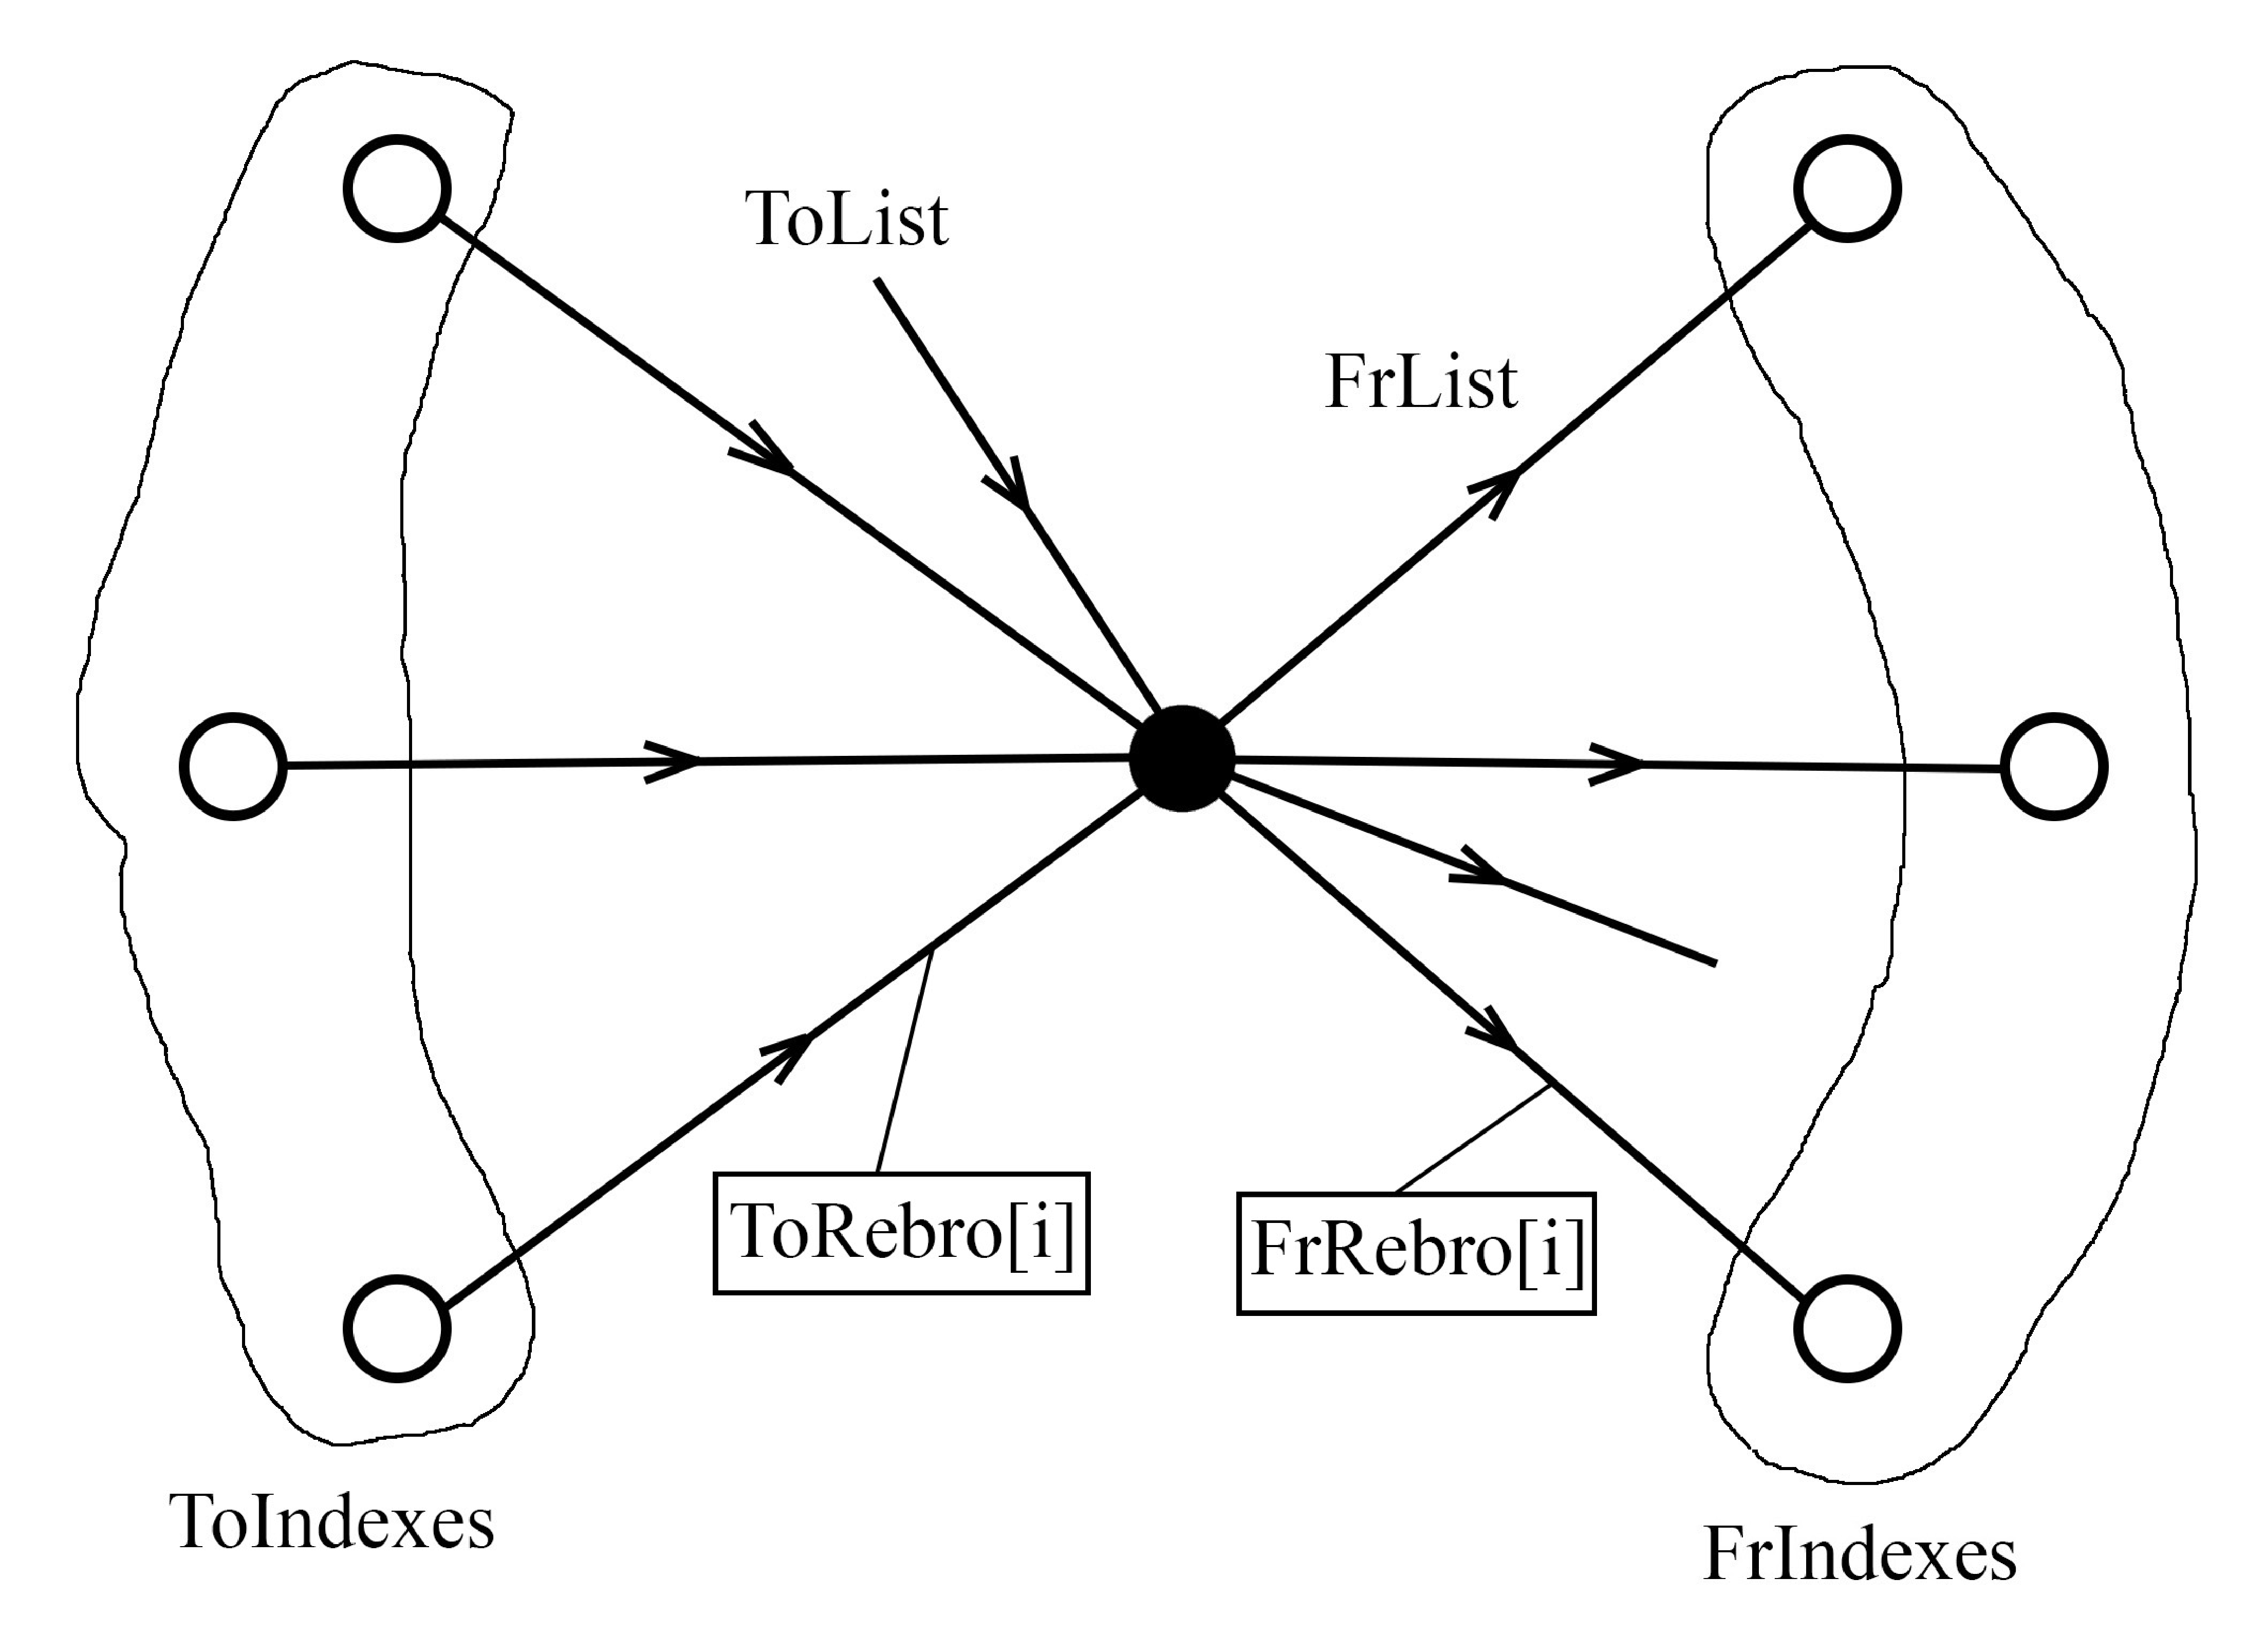
\includegraphics[width=1.0\linewidth]{Uzel_conn.eps}
\caption{\textsc{Схема связей для узла}}\label{fig61}
}
\end{figure}

В процессе анализа топологии расчётной схемы для узла составляются следующие списки:
\begin{enumerate}[topsep=5pt, itemsep=-3pt]
\item ToList --- список входящих в узел рёбер;
\item FrList --- список выходящих из узла рёбер;
\item UzelList --- список, содержащий имена данного узла и всех связанных с ним узлов;
\item ToIndexes --- список, содержащий локальные номера узлов из списка ToList;
\item FrIndexes --- список, содержащий локальные номера узлов из списка FrList,
\end{enumerate}
а также массив cJac глобальных номеров узлов из списка UzelList.

Запишем уравнения сохранения импульса для последних гидравлических связей рёбер, входящих в рассматриваемый узел:
\begin{equation}
\label{formula625}
(A_N^G)_{k_1} \cdot (\Delta(dP_{N-1}^n))_{k_1}+(B_N^G)_{k_1} \cdot (\Delta(dG_N^n))_{k_1} + (C_N^G)_{k_1} \cdot \Delta(dP_u^n)  = (-F_N^G)_{k_1}, 
\end{equation}
где $k_1$ --- номер входящего ребра; $N-1$ --- номер последней расчётной ячейки входящего в узел ребра; $N$ --- номер последней гидравлической связи входящего в узел ребра; $dP_u^n$ --- давление в рассматриваемом узле.

Запишем уравнения сохранения импульса для первых гидравлических связей рёбер, выходящих из рассматриваемого узла:
\begin{equation}
\label{formula626}
(A_0^G)_{k_2} \cdot \Delta(dP_u^n)+(B_0^G)_{k_2} \cdot (\Delta(dG_0^n))_{k_2} + (C_0^G)_{k_2} \cdot (\Delta(dP_0^n))_{k_2}  = (-F_0^G)_{k_2}, 
\end{equation}  
где $k_2$ --- номер выходящего ребра; $0$ --- номер первой ячейки выходящего из узла ребра и номер первой гидравлической связи.

Подставим в уравнения сохранения импульса вместо давлений в ячейках, примыкающих к узлу, их выражения через давления во входном и выходном узлах канала. Тогда для входящих рёбер получим
\begin{align}
\label{formula627}
&(A_N^G)_{k_1} \cdot \left[(S_{N-1}^0)_{k_1} + (S_{N-1}^1)_{k_1} \Delta(dP_{u_{in}}^n)_{k_1} + (S_{N-1}^2)_{k_1} \Delta(dP_u^n)\right]+(B_N^G)_{k_1} \cdot (\Delta(dG_N^n))_{k_1}+\notag ~\\
& + (C_N^G)_{k_1} \cdot \Delta(dP_u^n) = (-F_N^G)_{k_1}, 
\end{align}
а для выходящих рёбер ---
\begin{align}
\label{formula628}
&(A_0^G)_{k_2} \cdot \Delta(dP_u^n)+(B_0^G)_{k_2} \cdot (\Delta(dG_0^n))_{k_2} + \notag ~\\
& + (C_0^G)_{k_2} \cdot \left[(S_0^0)_{k_2} + (S_0^1)_{k_2} \Delta(dP_u^n) + (S_0^2)_{k_2} \Delta(dP_{u_{out}}^n)_{k_2}\right]  = (-F_0^G)_{k_2}, 
\end{align}
где $(dP_{u_{in}}^n)_{k_1}$ --- давление в узле на входе в $k_1$-е входящее ребро, а $(dP_{u_{out}}^n)_{k_2}$ --- давление в узле на выходе из $k_2$-го выходящего ребра. 

Выразим из полученных уравнений расходы в гидравлических связях:
\begin{align}
\label{formula629}
(\Delta(dG_N^n))_{k_1} = \frac{1}{(B_N^G)_{k_1}}\cdot \Big[
(-F_N^G)_{k_1}-(A_N^G)_{k_1}\cdot \big[(S_{N-1}^0)_{k_1} + (S_{N-1}^1)_{k_1} \Delta(dP_{u_{in}}^n)_{k_1} + \notag ~\\
+ (S_{N-1}^2)_{k_1} \Delta(dP_u^n)\big] - (C_N^G)_{k_1} \Delta(dP_u^n)\Big]; \notag ~\\
(\Delta(dG_0^n))_{k_2} = \frac{1}{(B_0^G)_{k_2}}\cdot \Big[(-F_0^G)_{k_2} - (A_0^G)_{k_2} \Delta(dP_u^n) - \notag ~\\
- (C_0^G)_{k_2}\cdot \big[(S_0^0)_{k_2} + (S_0^1)_{k_2} \Delta(dP_u^n) + (S_0^2)_{k_2} \Delta(dP_{u_{out}}^n)_{k_2}\big] \Big].
\end{align}

Раскроем скобки и сгруппируем слагаемые с давлениями в узлах и все остальные. Получим
\begin{align}
\label{formula630}
(\Delta(dG_N^n))_{k_1} = \frac{1}{(B_N^G)_{k_1}}\cdot \Big[[(-F_N^G)_{k_1}-(A_N^G)_{k_1}(S_{N-1}^0)_{k_1}]-(A_N^G)_{k_1}(S_{N-1}^1)_{k_1} \Delta(dP_{u_{in}}^n)_{k_1}-\notag ~\\
-[(A_N^G)_{k_1}(S_{N-1}^2)_{k_1}+(C_N^G)_{k_1}] \Delta(dP_u^n)      \Big]; \notag ~\\
(\Delta(dG_0^n))_{k_2} = \frac{1}{(B_0^G)_{k_2}}\cdot \Big[[(-F_0^G)_{k_2}-(C_0^G)_{k_2}(S_0^0)_{k_2}]-[(A_0^G)_{k_2}+(C_0^G)_{k_2}(S_0^1)_{k_2}]\Delta(dP_u^n) - \notag ~\\
- (C_0^G)_{k_2}(S_0^2)_{k_2} \Delta(dP_{u_{out}}^n)_{k_2} \Big].
\end{align}

Подставим эти расходы в уравнение сохранения массы для узла вида~\eqref{formula518}
\begin{align}
\label{formula631}
\left(A_k^P \right)'\cdot \sum_{j=1}^{K1} \frac{1}{(B_N^G)_j}\cdot \Big[[(-F_N^G)_j-(A_N^G)_j(S_{N-1}^0)_j]-(A_N^G)_j(S_{N-1}^1)_j \Delta(dP_{u_{in}}^n)_j - \notag ~\\
-[(A_N^G)_j(S_{N-1}^2)_j+(C_N^G)_j] \Delta(dP_u^n) \Big] + \left(B_k^P \right)' \cdot \Delta(dP_u^n) + \notag ~\\ 
+ \left(C_k^P \right)'\cdot \sum_{j=1}^{K2} \frac{1}{(B_0^G)_j}\cdot \Big[[(-F_0^G)_j-(C_0^G)_j(S_0^0)_j]-[(A_0^G)_j+(C_0^G)_j(S_0^1)_j]\Delta(dP_u^n) - \notag ~\\
- (C_0^G)_j(S_0^2)_j \Delta(dP_{u_{out}}^n)_j \Big] = -\left(F_k^P \right)',
\end{align}
где $k$ --- номер рассматриваемого узла; $K1$ --- количество входящих в рассматриваемый узел рёбер; $K2$ --- количество выходящих из рассматриваемого узла рёбер.

Выделим из полученного уравнения члены перед давлениями в соседних узлах, перед давлением в данном узле, и свободный член. Тогда будем иметь:
\begin{itemize}[topsep=5pt, itemsep=-3pt]
\item множитель перед давлениями во входящих узлах
\begin{equation}
\label{formula632}
\left(A_k^P \right)_j^{*}=\left(A_k^P \right)' \cdot \frac{1}{(B_N^G)_j}\cdot\left[-(A_N^G)_j(S_{N-1}^1)_j\right];
\end{equation}
\item множитель перед давлениями в выходящих узлах
\begin{equation}
\label{formula633}
\left(C_k^P \right)_j^{*}=\left(C_k^P \right)' \cdot \frac{1}{(B_0^G)_j}\cdot\left[-(C_0^G)_j(S_0^2)_j\right];
\end{equation}
\item множитель перед давлением в рассматриваемом узле
\begin{align}
\label{formula634}
\left(B_k^P \right)^{*}=\left(B_k^P \right)'&+\left(A_k^P \right)'\cdot \sum_{j=1}^{K1} \frac{-1}{(B_N^G)_j}\cdot[(A_N^G)_j(S_{N-1}^2)_j+(C_N^G)_j] + \notag ~\\
&+ \left(C_k^P \right)'\cdot \sum_{j=1}^{K2} \frac{-1}{(B_0^G)_j}\cdot [(A_0^G)_j+(C_0^G)_j(S_0^1)_j];
\end{align}
\item свободный член
\begin{align}
\label{formula635}
\left(F_k^P \right)^{*}=\left(F_k^P \right)'&+\left(A_k^P \right)'\cdot \sum_{j=1}^{K1} \frac{-1}{(B_N^G)_j}\cdot[(F_N^G)_j+(A_N^G)_j(S_{N-1}^0)_j] + \notag ~\\
&+\left(C_k^P \right)'\cdot \sum_{j=1}^{K2} \frac{-1}{(B_0^G)_j}\cdot [(F_0^G)_j+(C_0^G)_j(S_0^0)_j]. 
\end{align}
\end{itemize} 

С использованием сокращённых обозначений~\eqref{formula632} -- \eqref{formula635} окончательно уравнение сохранения массы для узла запишем в виде
\begin{equation}
\label{formula636}
\sum_{j=1}^{K1}\left(A_k^P \right)_j^{*}\cdot\Delta(dP_{u_{in}}^n)_j  + \left(B_k^P \right)^{*} \cdot \Delta(dP_k^n) + \sum_{j=1}^{K2} \left(C_k^P \right)_j^{*}\cdot \Delta(dP_{u_{out}}^n)_j  = -\left(F_k^P \right)^{*}.
\end{equation}

Если записать эти уравнения для всех внутренних узлов схемы, то получится СЛАУ относитель давлений в узлах. Размер матрицы этой СЛАУ будет равен $n\times n$, где $n$ --- общее количество внутренних узлов в схеме. Ненулевыми в каждой строке этой матрицы будут члены, соответствующие тем узлам, с которыми связан узел этой строки, и член, соответствующий самому узлу этой строки. Если решить СЛАУ каким-либо способом, то найдём погрешности для давлений в узлах на $r$-й итерации на текущем шаге по времени.

По найденным погрешностям для давлений в узлах найдём по уравнениям~\eqref{formula623} погрешности для давлений во всех расчётных ячейках всех каналов. Затем по уравнениям метода Ньютона-Рафсона~\eqref{formula55} можно перейти на $(r+1)$-ю итерацию на текущем шаге по времени.

По утверждению автора диссертации \cite{DisserKORSAR} этот метод расчёта поля давления в контуре произвольной топологии, названный им "безытерационным"{}, "превосходит известные классические методы решения полной системы уравнений относительно давлений в расчётных ячейках разветвлённого контура циркуляции более чем на порядок по быстродействию".  
 
Например, в диссертации приводятся результаты сравнения быс\-тро\-дей\-стви\-я пре\-дло\-жен\-но\-го метода относительно метода разреженных матриц библиотеки NAG для условий, когда количество точек ветвления значительно меньше общего количества расчётных ячеек. Показано, что безытерационный метод расчёта поля давления приблизительно в 17 раз превосходит метод разреженных матриц библиотеки NAG, и этот показатель не зависит от количества расчётных ячеек.

Следует, однако, учитывать, что в диссертации метод предлагается для расчёта двухфазных течений по более сложной физической модели по сравнению с заложенной в теплогидравлический код SimInTech, и, кроме того, там не рассматривается использование итерационного метода Ньютона-Рафсона (или какого-либо другого) для определения искомых величин на каждом шаге по времени. Одним словом, вопрос быстродействия метода требует отдельного исследования.    






 





\newpage

